\begin{center}
\Huge
Trigonometriske funktioner og harmoniske svinginger
\end{center}
\section*{Grader og radianer}
\stepcounter{section}

Vi har tidligere arbejdet med radianer i stedet for grader. Vi vil dog lige huske os selv på, hvordan det er radianer og grader hænger sammen. Som bekendt er omkredsen af enhedscirklen $2\pi$, så idéen er følgende: I stedet for at repræsentere en vinkel med gradtal, så repræsenteres den af længden af det linjestykke, vinkel overdækker på enhedscirklen. Idéen kan ses af Fig. \ref{fig:enhedscirkel}.
\begin{figure}[h]
	\centering
	\begin{tikzpicture}
		\draw (0,0) circle (4cm);
		\draw[-{Stealth[scale = 1.3]}] (-5,0) -- (5,0);
		\draw[-{Stealth[scale = 1.3]}] (0,-5) -- (0,5);
		\node at (3.1,3.1) {$\frac{\pi}{4}$};
		\node at (3.7,2.2) {$\frac{\pi}{6}$};
		\node at (2.2,3.7) {$\frac{\pi}{3}$};
		\node at (0.25,4.25)  {$\frac{\pi}{2}$};
		\node at (-3.1,3.1) {$\frac{3\pi}{4}$};
		\node at (-3.1,-3.1) {$\frac{5\pi}{4}$};
		\node at (3.1,-3.1) {$\frac{7\pi}{4}$};
		\node at (-3.7,2.2) {$\frac{5\pi}{6}$};
		\node at (-3.7,-2.2) {$\frac{7\pi}{6}$};
		\node at (3.7,-2.2) {$\frac{11\pi}{6}$};
		\node at (-2.2,3.7) {$\frac{2\pi}{3}$};
		\node at (-2.2,-3.7) {$\frac{4\pi}{3}$};
		\node at (2.2,-3.7) {$\frac{5\pi}{3}$};
		\node at (-4.25,0.25) {$\pi$};
		\node at (0.25,-4.25) {$\frac{3\pi}{2}$};
		\draw (0,0) -- (2.85,2.85);
		\draw (0,0) -- (3.5,2.05);
		\draw (0,0) -- (2.05,3.5);
		\draw (0,0) -- (-2.85,2.85);
		\draw (0,0) -- (-2.85,-2.85);
		\draw (0,0) -- (2.85,-2.85);
		\draw (0,0) -- (-3.5,2.05);
		\draw (0,0) -- (-3.5,-2.05);
		\draw (0,0) -- (3.5,-2.05);
		\draw (0,0) -- (-2.05,3.5);
		\draw (0,0) -- (-2.05,-3.5);
		\draw (0,0) -- (2.05,-3.5);
	\end{tikzpicture}
	\caption{Radianer tilsvarende bestemte vinkler.}
	\label{fig:enhedscirkel}
\end{figure}

\begin{setn}
Har vi en vinkel $v$ i grader og skal omregne til radianer, så er fremgangsmåden
\begin{align*}
	v\textnormal{ i grader} &\mapsto v \textnormal{ i radianer}\\
	v &\mapsto v\cdot \frac{2\pi}{360}.
\end{align*}
Har vi en vinkel $v$ i radianer og skal omregne til grader, så udregner vi:
\begin{align*}
	v\textnormal{ i radianer} &\mapsto v \textnormal{ i grader}\\
	v &\mapsto v\cdot \frac{360}{2\pi}.
\end{align*}
\end{setn}

\begin{exa}
	En vinkel er $180^\circ$. I radianer er den derfor 
	\begin{align*}
		180\cdot \frac{2\pi}{360} = \pi
	\end{align*}
	radianer. 
\end{exa}
\begin{exa}
	En vinkel er $\frac{2\pi}{3}$ radianer. Vi omregner til grader:
	\begin{align*}
		\frac{2\pi}{3} \cdot \frac{360}{2\pi} = 120^\circ.
	\end{align*}
\end{exa}

\section*{Harmoniske svingninger}
Vi vil - hvis andet ikke er nævnt - altid i forbindelse med de trigonometriske funktioner $\cos$, $\sin$ og $\tan$ bruge radianer og ikke grader. Vi er nu derfor at specificere definitionsmængde og dispositionsmængde for de trigonometriske funktioner. Cosinus er derfor funktionen $$\cos : \mathbb{R} \to [-1,1]$$
, sinus er funktionen 
$$\sin:\mathbb{R} \to [-1,1]$$ 
og tangens er funktionen
 $$\tan : 
\left\{x\in \mathbb{R}\ \middle| \  \frac{x}{\pi} + \frac{1}{2}\ \notin \mathbb{Z}  \right\} \to \mathbb{R}$$,
hvor funktionerne er givet som sædvanligt.


De trigonometriske funktioner $\cos(x)$ og $\sin(x)$ er periodiske funktioner, da 
\begin{align*}
\cos(x + 2\pi k) = \cos(x) 
\end{align*}
for alle heltal $k\in \mathbb{Z}$ og tilsvarende
\begin{align*}
\sin(x + 2\pi k) = \sin(x)
\end{align*}
for alle heltal $k$. Vi kan plotte $\cos(x)$ og $\sin(x)$, hvilket kan ses af Fig. \ref{fig:trig}

\begin{figure}[H]
\centering
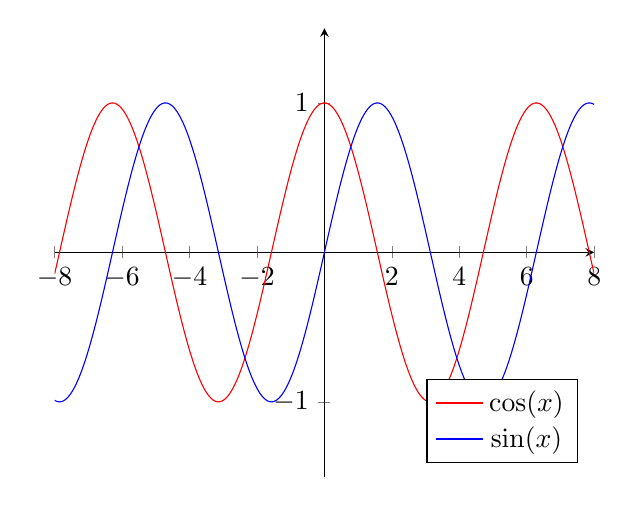
\begin{tikzpicture}
\begin{axis}[
axis lines = middle, 
xmin = -8, xmax = 8,
ymin = -1.5, ymax = 1.5,
legend pos = south east
]
\addplot[samples = 1000, color = red, domain = -8:8] {cos(deg(x))};
\addplot[samples = 1000, color = blue, domain = -8:8] {sin(deg(x))};
\legend{$\cos(x)$, $\sin(x)$}
\end{axis}
\end{tikzpicture}
\caption{Grafer for $\cos(x)$ og $\sin(x)$.}
\label{fig:trig}
\end{figure}

Som vi kan se af Fig \ref{fig:trig}, så er trigonometriske funktioner så langt fra injektive, som en funktion nærmest kan være. Til enhver funktionsværdi $f(x)$ tilhører der uendeligt mange $x$-værdier. Dog er $\cos$ og $\sin$ så vigtige, at vi gerne vil have en slags invers funktion til dem. Vi definerer derfor $$\cos : [0, \pi] \to [-1,1].$$ Denne funktion er surjektiv og injektiv, og vi kan derfor definere en invers funktion 
$$\cos^{-1} : [-1,1] \to [0,\pi].$$ 
Den kaldes også til tider for $\arccos$. Tilsvarende kan vi definere 
\begin{align*}
	\sin : [-\frac{\pi}{2},\frac{\pi}{2}] \to [-1,1].
\end{align*}
Den inverse funktion er så defineret
\begin{align*}
	\sin^{-1} : [-1,1] \to [-\frac{\pi}{2}, \frac{\pi}{2}],
\end{align*}
og kaldes til tider for $\arcsin$. 

\begin{exa}
	Vi har, at $\cos^{-1}(1) = 0,$ da $\cos(0) = 1$.
\end{exa}
Vi kan bruge trigonometriske funktioner til at modellere mange virkelige fænomener, da de er periodiske i natur. Vi kan eksempelvis bruge trigonometriske funktioner til at beskrive lyd og billedsignaler.

Da alle virkelige fænomener ikke har en periode på $2\pi$, så vil vi gerne kunne forkorte eller forlænge perioden. Vi vil også gerne kunne forskyde perioden, og vi vil gerne kunne øge \textit{amplituden}, så funktionen ikke kun går fra -1 til 1, men kan gå mellem større værdier. Desuden gælder der, at $\cos(x) = \sin(x + \frac{\pi}{2})$, så vi kan altid bruge $\sin$ til at beskrive $\cos$ og vice versa. Derfor giver vi følgende definition:
\begin{defn}[Harmoniske svingninger]
En sammenhæng 
\begin{align*}
y = A\cdot \sin(\omega t + \varphi)
\end{align*}
kaldes for en harmonisk svingning som funktion af tiden $t$. Konstanten $\omega$ kaldes for vinkelhastigheden, konstanten $\varphi$ kaldes for begyndelsesfasen og konstanten $A$ kaldes for amplituden. 
\end{defn}

\section*{Opgave 1}
Omregn følgende vinkler fra grader til radianer:
\begin{align*}
&1) \  90   &&2) \  180 \\
&3) \  130   &&4) \ 360  
\end{align*} 

\section*{Opgave 2}
Omregn følgende vinkler fra radianer til grader:
\begin{align*}
&1) \  2\pi  &&2) \  \frac{\pi}{4}    \\
&3) \  \frac{3\pi}{2}  &&4) \  \frac{\pi}{3}    
\end{align*}

\section*{Opgave 3}
Bestem følgende 
\begin{align*}
&1) \ \cos(\pi)    &&2) \ \sin(\pi/2)    \\
&3) \ \sin(45^\circ)    &&4) \ \cos(2\pi)    \\
\end{align*}

\section*{Opgave 4}
Bestem følgende
\begin{align*}
	&1) \ \cos^{-1}(0) &&2) \ \sin^{-1}(0) \\
	&2) \ \sin^{-1}(1) &&4) \ \cos^{-1}(\sqrt{2}/2)
\end{align*}
\section*{Opgave 5}
I Geogebra tegn så funktionen 
\begin{align*}
y = A\sin(\omega x + \varphi).
\end{align*}
\begin{enumerate}[label=\roman*)]
\item Hvordan ændrer det på grafen for sammenhængen at ændre på $\varphi$?
\item Hvordan ændrer det på grafen at ændre på $\omega$?
\item Hvordan ændrer det på grafen at ændre på $A$?
\end{enumerate}

\section*{Opgave 6}
I Geogebra tegn så $\cos(x)$ og $\sin(x+k)$, og bestem $k$, så graferne er sammenfaldende. Argumentér ved brug af enhedscirklen for, at graferne er sammenfaldende i dette tilfælde. 

\section*{Opgave 7}
Vi kan ved en bestemt havn modellere vandstanden med den harmoniske svingning
\begin{align*}
f(t) = 1.2\sin(0.524t) + 3.4,
\end{align*}
hvor $t$ er tiden målt i timer og $f(t)$ er vandstanden i meter. 
\begin{enumerate}[label=\roman*)]
\item Tegn grafen for $f$ i Geogebra. 
\item På hvor mange timer er en periode? (Antallet af timer, før vandstanden er det samme igen)
\item Hvornår er vandstanden højest? Hvad med lavest?
\end{enumerate}


